% Options for packages loaded elsewhere
\PassOptionsToPackage{unicode}{hyperref}
\PassOptionsToPackage{hyphens}{url}
\documentclass[
]{article}
\usepackage{xcolor}
\usepackage[margin=1in]{geometry}
\usepackage{amsmath,amssymb}
\setcounter{secnumdepth}{-\maxdimen} % remove section numbering
\usepackage{iftex}
\ifPDFTeX
  \usepackage[T1]{fontenc}
  \usepackage[utf8]{inputenc}
  \usepackage{textcomp} % provide euro and other symbols
\else % if luatex or xetex
  \usepackage{unicode-math} % this also loads fontspec
  \defaultfontfeatures{Scale=MatchLowercase}
  \defaultfontfeatures[\rmfamily]{Ligatures=TeX,Scale=1}
\fi
\usepackage{lmodern}
\ifPDFTeX\else
  % xetex/luatex font selection
\fi
% Use upquote if available, for straight quotes in verbatim environments
\IfFileExists{upquote.sty}{\usepackage{upquote}}{}
\IfFileExists{microtype.sty}{% use microtype if available
  \usepackage[]{microtype}
  \UseMicrotypeSet[protrusion]{basicmath} % disable protrusion for tt fonts
}{}
\makeatletter
\@ifundefined{KOMAClassName}{% if non-KOMA class
  \IfFileExists{parskip.sty}{%
    \usepackage{parskip}
  }{% else
    \setlength{\parindent}{0pt}
    \setlength{\parskip}{6pt plus 2pt minus 1pt}}
}{% if KOMA class
  \KOMAoptions{parskip=half}}
\makeatother
\usepackage{color}
\usepackage{fancyvrb}
\newcommand{\VerbBar}{|}
\newcommand{\VERB}{\Verb[commandchars=\\\{\}]}
\DefineVerbatimEnvironment{Highlighting}{Verbatim}{commandchars=\\\{\}}
% Add ',fontsize=\small' for more characters per line
\usepackage{framed}
\definecolor{shadecolor}{RGB}{248,248,248}
\newenvironment{Shaded}{\begin{snugshade}}{\end{snugshade}}
\newcommand{\AlertTok}[1]{\textcolor[rgb]{0.94,0.16,0.16}{#1}}
\newcommand{\AnnotationTok}[1]{\textcolor[rgb]{0.56,0.35,0.01}{\textbf{\textit{#1}}}}
\newcommand{\AttributeTok}[1]{\textcolor[rgb]{0.13,0.29,0.53}{#1}}
\newcommand{\BaseNTok}[1]{\textcolor[rgb]{0.00,0.00,0.81}{#1}}
\newcommand{\BuiltInTok}[1]{#1}
\newcommand{\CharTok}[1]{\textcolor[rgb]{0.31,0.60,0.02}{#1}}
\newcommand{\CommentTok}[1]{\textcolor[rgb]{0.56,0.35,0.01}{\textit{#1}}}
\newcommand{\CommentVarTok}[1]{\textcolor[rgb]{0.56,0.35,0.01}{\textbf{\textit{#1}}}}
\newcommand{\ConstantTok}[1]{\textcolor[rgb]{0.56,0.35,0.01}{#1}}
\newcommand{\ControlFlowTok}[1]{\textcolor[rgb]{0.13,0.29,0.53}{\textbf{#1}}}
\newcommand{\DataTypeTok}[1]{\textcolor[rgb]{0.13,0.29,0.53}{#1}}
\newcommand{\DecValTok}[1]{\textcolor[rgb]{0.00,0.00,0.81}{#1}}
\newcommand{\DocumentationTok}[1]{\textcolor[rgb]{0.56,0.35,0.01}{\textbf{\textit{#1}}}}
\newcommand{\ErrorTok}[1]{\textcolor[rgb]{0.64,0.00,0.00}{\textbf{#1}}}
\newcommand{\ExtensionTok}[1]{#1}
\newcommand{\FloatTok}[1]{\textcolor[rgb]{0.00,0.00,0.81}{#1}}
\newcommand{\FunctionTok}[1]{\textcolor[rgb]{0.13,0.29,0.53}{\textbf{#1}}}
\newcommand{\ImportTok}[1]{#1}
\newcommand{\InformationTok}[1]{\textcolor[rgb]{0.56,0.35,0.01}{\textbf{\textit{#1}}}}
\newcommand{\KeywordTok}[1]{\textcolor[rgb]{0.13,0.29,0.53}{\textbf{#1}}}
\newcommand{\NormalTok}[1]{#1}
\newcommand{\OperatorTok}[1]{\textcolor[rgb]{0.81,0.36,0.00}{\textbf{#1}}}
\newcommand{\OtherTok}[1]{\textcolor[rgb]{0.56,0.35,0.01}{#1}}
\newcommand{\PreprocessorTok}[1]{\textcolor[rgb]{0.56,0.35,0.01}{\textit{#1}}}
\newcommand{\RegionMarkerTok}[1]{#1}
\newcommand{\SpecialCharTok}[1]{\textcolor[rgb]{0.81,0.36,0.00}{\textbf{#1}}}
\newcommand{\SpecialStringTok}[1]{\textcolor[rgb]{0.31,0.60,0.02}{#1}}
\newcommand{\StringTok}[1]{\textcolor[rgb]{0.31,0.60,0.02}{#1}}
\newcommand{\VariableTok}[1]{\textcolor[rgb]{0.00,0.00,0.00}{#1}}
\newcommand{\VerbatimStringTok}[1]{\textcolor[rgb]{0.31,0.60,0.02}{#1}}
\newcommand{\WarningTok}[1]{\textcolor[rgb]{0.56,0.35,0.01}{\textbf{\textit{#1}}}}
\usepackage{graphicx}
\makeatletter
\newsavebox\pandoc@box
\newcommand*\pandocbounded[1]{% scales image to fit in text height/width
  \sbox\pandoc@box{#1}%
  \Gscale@div\@tempa{\textheight}{\dimexpr\ht\pandoc@box+\dp\pandoc@box\relax}%
  \Gscale@div\@tempb{\linewidth}{\wd\pandoc@box}%
  \ifdim\@tempb\p@<\@tempa\p@\let\@tempa\@tempb\fi% select the smaller of both
  \ifdim\@tempa\p@<\p@\scalebox{\@tempa}{\usebox\pandoc@box}%
  \else\usebox{\pandoc@box}%
  \fi%
}
% Set default figure placement to htbp
\def\fps@figure{htbp}
\makeatother
\setlength{\emergencystretch}{3em} % prevent overfull lines
\providecommand{\tightlist}{%
  \setlength{\itemsep}{0pt}\setlength{\parskip}{0pt}}
\usepackage{fontspec}
\setmainfont{Times New Roman}  % Replace with a Unicode-friendly font installed on your system
\usepackage{bookmark}
\IfFileExists{xurl.sty}{\usepackage{xurl}}{} % add URL line breaks if available
\urlstyle{same}
\hypersetup{
  pdftitle={Imports ARIMA},
  pdfauthor={Andrew Jowe},
  hidelinks,
  pdfcreator={LaTeX via pandoc}}

\title{Imports ARIMA}
\author{Andrew Jowe}
\date{}

\begin{document}
\maketitle

\section{Col Removal}\label{col-removal}

Keep Year, Imports, and GDP columns

\begin{Shaded}
\begin{Highlighting}[]
\NormalTok{finalPro\_data }\OtherTok{\textless{}{-}}\NormalTok{ finalPro\_data[, }\FunctionTok{c}\NormalTok{(}\StringTok{"Year"}\NormalTok{, }\StringTok{"Imports"}\NormalTok{)]}
\end{Highlighting}
\end{Shaded}

\section{Plot Time Series}\label{plot-time-series}

\begin{Shaded}
\begin{Highlighting}[]
\CommentTok{\# Plot Imports}
\NormalTok{imports\_ts }\OtherTok{\textless{}{-}} \FunctionTok{ts}\NormalTok{(finalPro\_data}\SpecialCharTok{$}\NormalTok{Imports, }\AttributeTok{start =} \DecValTok{1960}\NormalTok{, }\AttributeTok{frequency =} \DecValTok{1}\NormalTok{)}

\FunctionTok{ts.plot}\NormalTok{(imports\_ts, }\AttributeTok{main=}\StringTok{"Imports Time Series"}\NormalTok{, }\AttributeTok{ylab=}\StringTok{"Imports"}\NormalTok{)}
\end{Highlighting}
\end{Shaded}

\pandocbounded{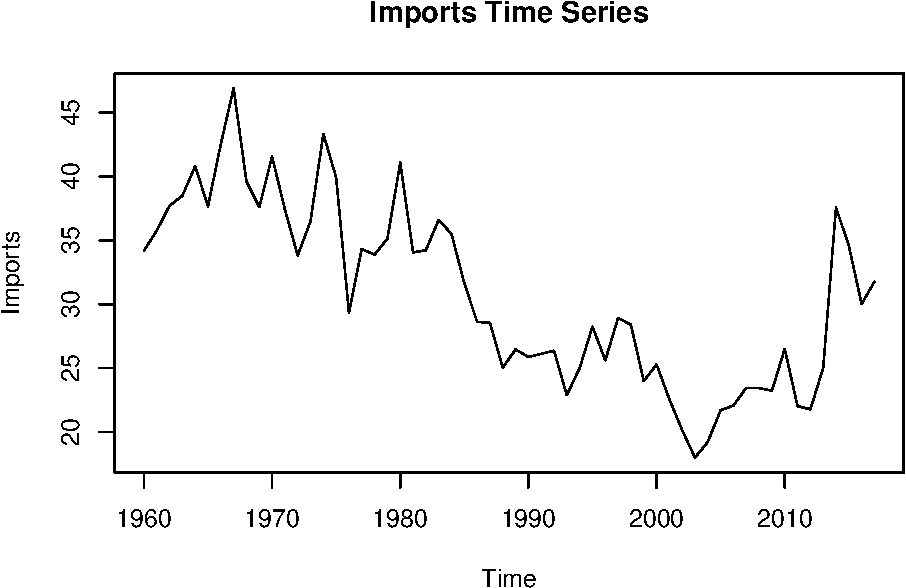
\includegraphics[keepaspectratio]{final_imports_files/figure-latex/unnamed-chunk-3-1.pdf}}

Summary: - Imports time series has upward trend, this shows this is
non-stationary - It has peaks around every 10 year: 1980, 1990, 2010

\section{Transform}\label{transform}

\begin{Shaded}
\begin{Highlighting}[]
\CommentTok{\# Box{-}Cox transform Imports}
\NormalTok{lambda }\OtherTok{\textless{}{-}} \FunctionTok{BoxCox.lambda}\NormalTok{(imports\_ts)}
\NormalTok{boxcox\_imports\_ts }\OtherTok{\textless{}{-}} \FunctionTok{BoxCox}\NormalTok{(imports\_ts, lambda)}
\FunctionTok{ts.plot}\NormalTok{(boxcox\_imports\_ts, }\AttributeTok{main =} \FunctionTok{paste}\NormalTok{(}\StringTok{"Box{-}Cox Transformed Imports (lambda ="}\NormalTok{, }\FunctionTok{round}\NormalTok{(lambda, }\DecValTok{3}\NormalTok{), }\StringTok{")"}\NormalTok{), }\AttributeTok{ylab =} \StringTok{"Transformed Imports"}\NormalTok{)}
\end{Highlighting}
\end{Shaded}

\pandocbounded{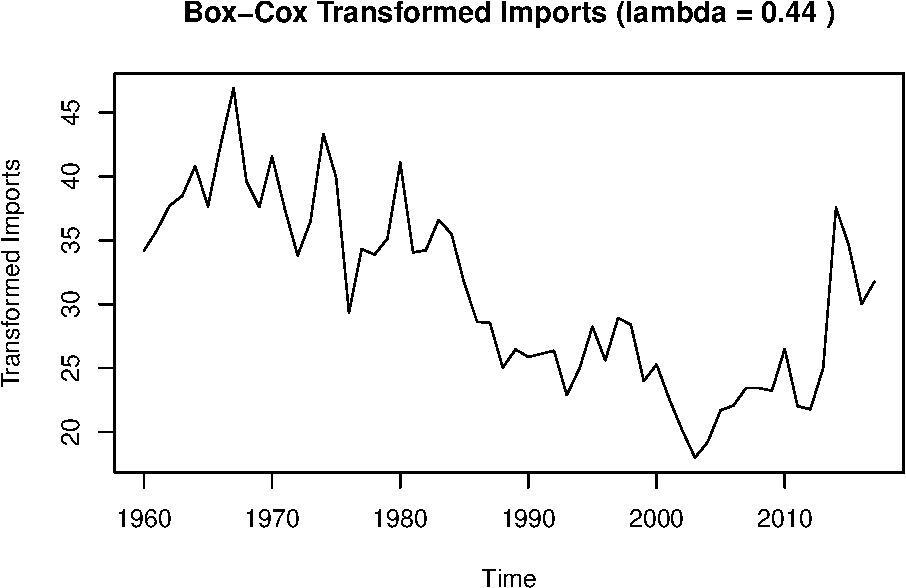
\includegraphics[keepaspectratio]{final_imports_files/figure-latex/unnamed-chunk-4-1.pdf}}

We tried log, but residuals not normal.

\section{Differencing Imports}\label{differencing-imports}

\begin{Shaded}
\begin{Highlighting}[]
\NormalTok{diff\_imports\_bc }\OtherTok{\textless{}{-}} \FunctionTok{diff}\NormalTok{(boxcox\_imports\_ts, }\AttributeTok{differences=}\DecValTok{2}\NormalTok{)}

\CommentTok{\# Plot differenced Box{-}Cox Imports}
\FunctionTok{ts.plot}\NormalTok{(diff\_imports\_bc, }\AttributeTok{main=}\StringTok{"Differenced Box{-}Cox Transformed Imports Time Series"}\NormalTok{, }\AttributeTok{ylab=}\StringTok{"Transformed Imports"}\NormalTok{)}
\end{Highlighting}
\end{Shaded}

\pandocbounded{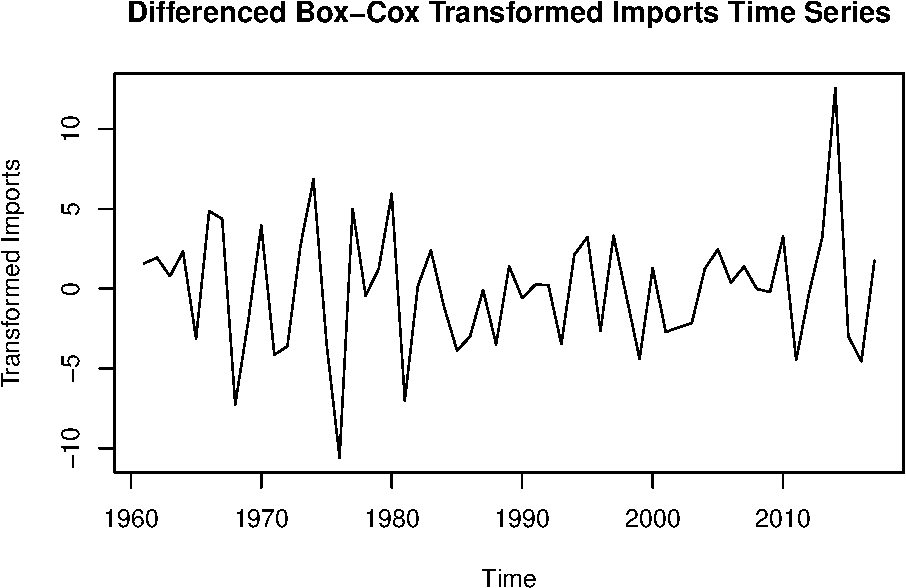
\includegraphics[keepaspectratio]{final_imports_files/figure-latex/unnamed-chunk-5-1.pdf}}

\section{ACF / PACF plots}\label{acf-pacf-plots}

\begin{Shaded}
\begin{Highlighting}[]
\CommentTok{\# ACF and PACF of the transformed and differenced series}
\FunctionTok{par}\NormalTok{(}\AttributeTok{mfrow =} \FunctionTok{c}\NormalTok{(}\DecValTok{1}\NormalTok{, }\DecValTok{2}\NormalTok{))}
\FunctionTok{Acf}\NormalTok{(diff\_imports\_bc, }\AttributeTok{main =} \StringTok{"ACF of Transformed + Differenced Series"}\NormalTok{)}
\FunctionTok{Pacf}\NormalTok{(diff\_imports\_bc, }\AttributeTok{main =} \StringTok{"PACF of Transformed + Differenced Series"}\NormalTok{)}
\end{Highlighting}
\end{Shaded}

\pandocbounded{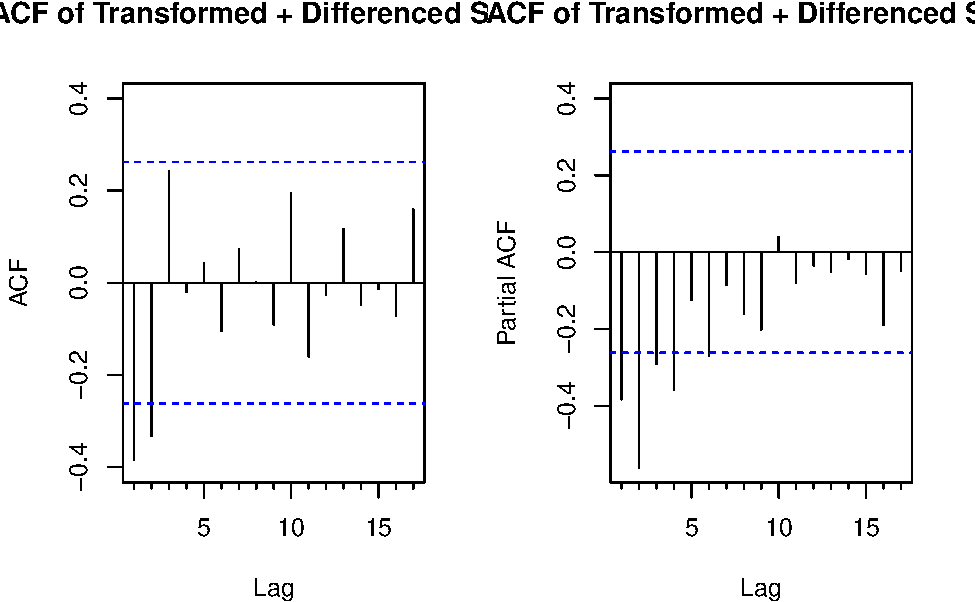
\includegraphics[keepaspectratio]{final_imports_files/figure-latex/unnamed-chunk-6-1.pdf}}

\begin{Shaded}
\begin{Highlighting}[]
\FunctionTok{par}\NormalTok{(}\AttributeTok{mfrow =} \FunctionTok{c}\NormalTok{(}\DecValTok{1}\NormalTok{, }\DecValTok{1}\NormalTok{))}
\end{Highlighting}
\end{Shaded}

\section{Modeling}\label{modeling}

\begin{Shaded}
\begin{Highlighting}[]
\CommentTok{\# Central African Republic Imports ARIMA Model}
\CommentTok{\# Author: Om C}

\CommentTok{\# Diagnostics on chosen model}
\NormalTok{final\_model }\OtherTok{\textless{}{-}} \FunctionTok{Arima}\NormalTok{(boxcox\_imports\_ts, }\AttributeTok{order =} \FunctionTok{c}\NormalTok{(}\DecValTok{2}\NormalTok{, }\DecValTok{2}\NormalTok{, }\DecValTok{4}\NormalTok{), }\AttributeTok{method =} \StringTok{"ML"}\NormalTok{)}
\FunctionTok{print}\NormalTok{(final\_model)}
\end{Highlighting}
\end{Shaded}

\begin{verbatim}
## Series: boxcox_imports_ts 
## ARIMA(2,2,4) 
## 
## Coefficients:
##          ar1     ar2      ma1      ma2     ma3      ma4
##       0.1315  0.0604  -1.2198  -0.2171  0.6705  -0.2336
## s.e.  2.2418  0.9942   2.2268   1.5518  1.6514   0.8995
## 
## sigma^2 = 0.2744:  log likelihood = -42.64
## AIC=99.27   AICc=101.61   BIC=113.45
\end{verbatim}

\begin{Shaded}
\begin{Highlighting}[]
\NormalTok{residuals\_final }\OtherTok{\textless{}{-}} \FunctionTok{residuals}\NormalTok{(final\_model)}

\CommentTok{\# Residual ACF and PACF for final model}
\FunctionTok{par}\NormalTok{(}\AttributeTok{mfrow =} \FunctionTok{c}\NormalTok{(}\DecValTok{1}\NormalTok{, }\DecValTok{2}\NormalTok{))  }\CommentTok{\# Side{-}by{-}side layout}
\FunctionTok{acf}\NormalTok{(residuals\_final, }\AttributeTok{main =} \StringTok{"ACF of Final Model Residuals"}\NormalTok{)}
\FunctionTok{pacf}\NormalTok{(residuals\_final, }\AttributeTok{main =} \StringTok{"PACF of Final Model Residuals"}\NormalTok{)}
\end{Highlighting}
\end{Shaded}

\pandocbounded{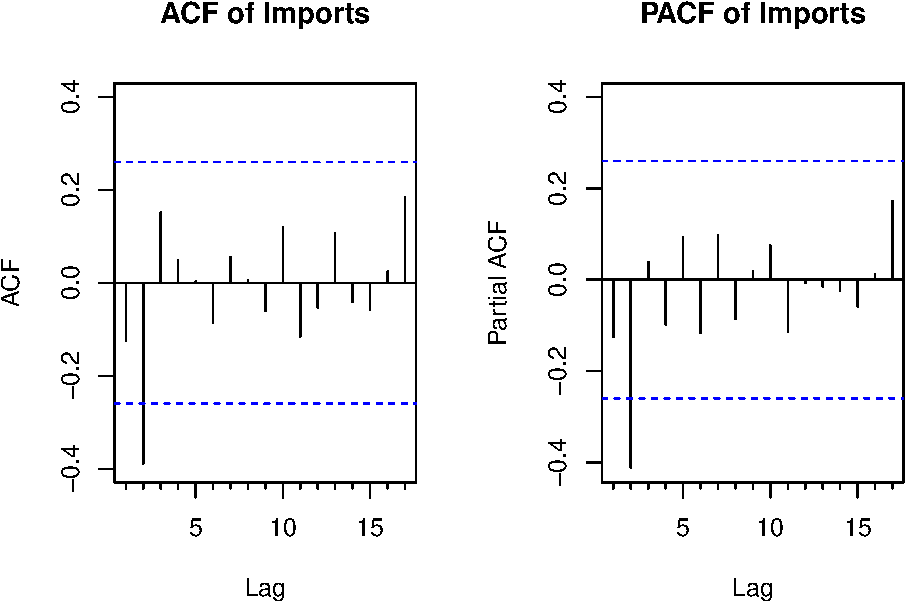
\includegraphics[keepaspectratio]{final_imports_files/figure-latex/unnamed-chunk-7-1.pdf}}

\begin{Shaded}
\begin{Highlighting}[]
\FunctionTok{par}\NormalTok{(}\AttributeTok{mfrow =} \FunctionTok{c}\NormalTok{(}\DecValTok{1}\NormalTok{, }\DecValTok{1}\NormalTok{))  }\CommentTok{\# Reset layout}

\CommentTok{\# Diagnostic Tests (Simplified)}
\FunctionTok{cat}\NormalTok{(}\StringTok{"}\SpecialCharTok{\textbackslash{}n}\StringTok{Diagnostic Tests (Simplified):}\SpecialCharTok{\textbackslash{}n}\StringTok{"}\NormalTok{)}
\end{Highlighting}
\end{Shaded}

\begin{verbatim}
## 
## Diagnostic Tests (Simplified):
\end{verbatim}

\begin{Shaded}
\begin{Highlighting}[]
\CommentTok{\# 1. Portmanteau (Ljung{-}Box) Test for Autocorrelation}
\NormalTok{ljung }\OtherTok{\textless{}{-}} \FunctionTok{Box.test}\NormalTok{(residuals\_final, }\AttributeTok{lag =} \DecValTok{10}\NormalTok{, }\AttributeTok{type =} \StringTok{"Ljung{-}Box"}\NormalTok{)}
\FunctionTok{cat}\NormalTok{(}\StringTok{"Ljung{-}Box test p{-}value:"}\NormalTok{, }\FunctionTok{round}\NormalTok{(ljung}\SpecialCharTok{$}\NormalTok{p.value, }\DecValTok{4}\NormalTok{), }
    \FunctionTok{ifelse}\NormalTok{(ljung}\SpecialCharTok{$}\NormalTok{p.value }\SpecialCharTok{\textgreater{}} \FloatTok{0.05}\NormalTok{, }\StringTok{"(PASS {-} residuals ≈ white noise)"}\NormalTok{, }\StringTok{"(FAIL)"}\NormalTok{), }\StringTok{"}\SpecialCharTok{\textbackslash{}n}\StringTok{"}\NormalTok{)}
\end{Highlighting}
\end{Shaded}

\begin{verbatim}
## Ljung-Box test p-value: 0.9991 (PASS - residuals ≈ white noise)
\end{verbatim}

\begin{Shaded}
\begin{Highlighting}[]
\CommentTok{\# 2. Shapiro{-}Wilk Test for Normality}
\CommentTok{\# this does not violate model assumptions, but it violates confidence interval assumptions}
\NormalTok{shapiro }\OtherTok{\textless{}{-}} \FunctionTok{shapiro.test}\NormalTok{(residuals\_final)}
\FunctionTok{cat}\NormalTok{(}\StringTok{"Shapiro{-}Wilk test p{-}value:"}\NormalTok{, }\FunctionTok{round}\NormalTok{(shapiro}\SpecialCharTok{$}\NormalTok{p.value, }\DecValTok{4}\NormalTok{), }
    \FunctionTok{ifelse}\NormalTok{(shapiro}\SpecialCharTok{$}\NormalTok{p.value }\SpecialCharTok{\textgreater{}} \FloatTok{0.05}\NormalTok{, }\StringTok{"(PASS {-} approx. normal residuals)"}\NormalTok{, }\StringTok{"(FAIL)"}\NormalTok{), }\StringTok{"}\SpecialCharTok{\textbackslash{}n}\StringTok{"}\NormalTok{)}
\end{Highlighting}
\end{Shaded}

\begin{verbatim}
## Shapiro-Wilk test p-value: 0.002 (FAIL)
\end{verbatim}

\begin{Shaded}
\begin{Highlighting}[]
\CommentTok{\# STEP 3: Model Comparison}
\CommentTok{\# Expanded grid search from ARIMA(0,2,0) to ARIMA(8,2,8)}
\NormalTok{models }\OtherTok{\textless{}{-}} \FunctionTok{list}\NormalTok{()}
\ControlFlowTok{for}\NormalTok{ (p }\ControlFlowTok{in} \DecValTok{0}\SpecialCharTok{:}\DecValTok{8}\NormalTok{) \{}
  \ControlFlowTok{for}\NormalTok{ (q }\ControlFlowTok{in} \DecValTok{0}\SpecialCharTok{:}\DecValTok{8}\NormalTok{) \{}
\NormalTok{    name }\OtherTok{\textless{}{-}} \FunctionTok{paste0}\NormalTok{(}\StringTok{"ARIMA("}\NormalTok{, p, }\StringTok{",2,"}\NormalTok{, q, }\StringTok{")"}\NormalTok{)}
\NormalTok{    models[[name]] }\OtherTok{\textless{}{-}} \FunctionTok{c}\NormalTok{(p, }\DecValTok{2}\NormalTok{, q)}
\NormalTok{  \}}
\NormalTok{\}}
\NormalTok{results }\OtherTok{\textless{}{-}} \FunctionTok{data.frame}\NormalTok{(}\AttributeTok{Model=}\FunctionTok{character}\NormalTok{(), }\AttributeTok{AIC=}\FunctionTok{numeric}\NormalTok{(), }\AttributeTok{BIC=}\FunctionTok{numeric}\NormalTok{(), }
                     \AttributeTok{Ljung\_Box\_p=}\FunctionTok{numeric}\NormalTok{(), }\AttributeTok{stringsAsFactors=}\ConstantTok{FALSE}\NormalTok{)}

\ControlFlowTok{for}\NormalTok{(i }\ControlFlowTok{in} \DecValTok{1}\SpecialCharTok{:}\FunctionTok{length}\NormalTok{(models)) \{}
\NormalTok{  fit }\OtherTok{\textless{}{-}} \FunctionTok{Arima}\NormalTok{(boxcox\_imports\_ts, }\AttributeTok{order =}\NormalTok{ models[[i]], }\AttributeTok{method =} \StringTok{"ML"}\NormalTok{)}
\NormalTok{  ljung\_p }\OtherTok{\textless{}{-}} \FunctionTok{Box.test}\NormalTok{(}\FunctionTok{residuals}\NormalTok{(fit), }\AttributeTok{lag =} \DecValTok{10}\NormalTok{, }\AttributeTok{type =} \StringTok{"Ljung{-}Box"}\NormalTok{)}\SpecialCharTok{$}\NormalTok{p.value}
\NormalTok{  results }\OtherTok{\textless{}{-}} \FunctionTok{rbind}\NormalTok{(results, }\FunctionTok{data.frame}\NormalTok{(}
    \AttributeTok{Model =} \FunctionTok{names}\NormalTok{(models)[i],}
    \AttributeTok{AIC =}\NormalTok{ fit}\SpecialCharTok{$}\NormalTok{aic,}
    \AttributeTok{BIC =} \FunctionTok{BIC}\NormalTok{(fit),}
    \AttributeTok{Ljung\_Box\_p =}\NormalTok{ ljung\_p}
\NormalTok{  ))}
\NormalTok{\}}
\FunctionTok{print}\NormalTok{(results)}
\end{Highlighting}
\end{Shaded}

\begin{verbatim}
##           Model       AIC      BIC Ljung_Box_p
## 1  ARIMA(0,2,0) 137.28956 139.3149 0.007392716
## 2  ARIMA(0,2,1)  98.92003 102.9707 0.300984142
## 3  ARIMA(0,2,2)  99.56537 105.6414 0.603473280
## 4  ARIMA(0,2,3)  94.40791 102.5093 0.972310042
## 5  ARIMA(0,2,4)  95.44415 105.5709 0.998840481
## 6  ARIMA(0,2,5)  97.41561 109.5677 0.999429054
## 7  ARIMA(0,2,6)  99.27038 113.4478 0.999063945
## 8  ARIMA(0,2,7)  99.03487 115.2377 0.999882225
## 9  ARIMA(0,2,8) 100.87092 119.0991 0.999469161
## 10 ARIMA(1,2,0) 130.34115 134.3919 0.007983749
## 11 ARIMA(1,2,1) 100.44891 106.5250 0.379433823
## 12 ARIMA(1,2,2)  99.74612 107.8475 0.640864630
## 13 ARIMA(1,2,3)  95.42107 105.5478 0.999390955
## 14 ARIMA(1,2,4)  97.28056 109.4327 0.998896565
## 15 ARIMA(1,2,5)  99.28015 113.4576 0.998979211
## 16 ARIMA(1,2,6) 100.67512 116.8779 0.995637188
## 17 ARIMA(1,2,7) 103.16947 121.3976 0.999458141
## 18 ARIMA(1,2,8) 100.88320 121.1367 0.999934133
## 19 ARIMA(2,2,0) 111.04723 117.1233 0.328463169
## 20 ARIMA(2,2,1)  94.67868 102.7801 0.972608144
## 21 ARIMA(2,2,2)  96.39999 106.5268 0.977034139
## 22 ARIMA(2,2,3)  97.35797 109.5101 0.998899821
## 23 ARIMA(2,2,4)  99.27454 113.4520 0.999051801
## 24 ARIMA(2,2,5) 101.27079 117.4736 0.999078931
## 25 ARIMA(2,2,6) 102.24174 120.4699 0.999955567
## 26 ARIMA(2,2,7) 104.35120 124.6047 0.999988850
## 27 ARIMA(2,2,8) 102.41569 124.6946 0.999999871
## 28 ARIMA(3,2,0) 108.15716 116.2586 0.426049148
## 29 ARIMA(3,2,1)  96.53640 106.6632 0.969146347
## 30 ARIMA(3,2,2)  97.46473 109.6168 0.997628351
## 31 ARIMA(3,2,3)  99.29430 113.4718 0.999003493
## 32 ARIMA(3,2,4) 101.22256 117.4254 0.998928013
## 33 ARIMA(3,2,5) 101.09811 119.3263 0.999305795
## 34 ARIMA(3,2,6) 104.22521 124.4787 0.999969301
## 35 ARIMA(3,2,7) 104.23172 126.5106 0.999991950
## 36 ARIMA(3,2,8) 104.26123 128.5655 0.999999860
## 37 ARIMA(4,2,0) 102.85355 112.9803 0.824168012
## 38 ARIMA(4,2,1)  98.33486 110.4870 0.983885692
## 39 ARIMA(4,2,2)  99.13240 113.3099 0.999472679
## 40 ARIMA(4,2,3)  97.82297 114.0258 0.999992498
## 41 ARIMA(4,2,4)  99.57220 117.8004 0.999998608
## 42 ARIMA(4,2,5) 102.61541 122.8689 0.999939598
## 43 ARIMA(4,2,6) 106.14050 128.4194 0.999986401
## 44 ARIMA(4,2,7) 104.15488 128.4591 0.999956422
## 45 ARIMA(4,2,8) 104.65627 130.9858 0.999990864
## 46 ARIMA(5,2,0) 104.23982 116.3919 0.818517004
## 47 ARIMA(5,2,1)  99.66784 113.8453 0.992272386
## 48 ARIMA(5,2,2) 100.72691 116.9297 0.999610328
## 49 ARIMA(5,2,3)  99.53444 117.7626 0.999996370
## 50 ARIMA(5,2,4) 100.22313 120.4766 0.999997871
## 51 ARIMA(5,2,5) 103.48572 125.7646 0.999998334
## 52 ARIMA(5,2,6) 105.07517 129.3794 0.999579301
## 53 ARIMA(5,2,7) 104.23149 130.5611 0.999986852
## 54 ARIMA(5,2,8) 106.00338 134.3583 0.999993170
## 55 ARIMA(6,2,0) 102.89362 117.0711 0.990360288
## 56 ARIMA(6,2,1) 100.89835 117.1012 0.999694649
## 57 ARIMA(6,2,2) 102.49243 120.7206 0.999940556
## 58 ARIMA(6,2,3) 101.41813 121.6716 0.999998907
## 59 ARIMA(6,2,4) 103.52895 125.8078 0.999995414
## 60 ARIMA(6,2,5) 103.51166 127.8159 0.999998382
## 61 ARIMA(6,2,6) 104.53588 130.8655 0.999944765
## 62 ARIMA(6,2,7) 106.45401 134.8089 0.999953209
## 63 ARIMA(6,2,8) 107.82987 138.2101 0.999692338
## 64 ARIMA(7,2,0) 104.65618 120.8590 0.994041309
## 65 ARIMA(7,2,1) 102.61420 120.8424 0.999954079
## 66 ARIMA(7,2,2) 104.41178 124.6653 0.999979135
## 67 ARIMA(7,2,3) 104.18233 126.4612 0.999972309
## 68 ARIMA(7,2,4) 105.40533 129.7096 0.999999076
## 69 ARIMA(7,2,5) 104.90603 131.2356 0.999944099
## 70 ARIMA(7,2,6) 109.13207 137.4870 0.999997782
## 71 ARIMA(7,2,7) 107.79159 138.1719 0.999999872
## 72 ARIMA(7,2,8) 110.98788 143.3935 0.999895598
## 73 ARIMA(8,2,0) 104.94831 123.1765 0.994434645
## 74 ARIMA(8,2,1) 104.14180 124.3953 0.999997869
## 75 ARIMA(8,2,2) 106.25459 128.5335 0.999971253
## 76 ARIMA(8,2,3) 104.58804 128.8923 0.999999524
## 77 ARIMA(8,2,4) 107.97852 134.3081 0.999993818
## 78 ARIMA(8,2,5) 109.97704 138.3320 0.999994023
## 79 ARIMA(8,2,6) 109.16964 139.5499 0.999965489
## 80 ARIMA(8,2,7) 107.91277 140.3184 0.999865281
## 81 ARIMA(8,2,8) 111.68628 146.1173 0.999997283
\end{verbatim}

\begin{Shaded}
\begin{Highlighting}[]
\CommentTok{\# If we inspect the BIC too, the one with min AIC is likely to also have the min BIC}
\FunctionTok{cat}\NormalTok{(}\StringTok{"}\SpecialCharTok{\textbackslash{}n}\StringTok{Best model by AIC:"}\NormalTok{, results}\SpecialCharTok{$}\NormalTok{Model[}\FunctionTok{which.min}\NormalTok{(results}\SpecialCharTok{$}\NormalTok{AIC)], }\StringTok{"}\SpecialCharTok{\textbackslash{}n}\StringTok{"}\NormalTok{)}
\end{Highlighting}
\end{Shaded}

\begin{verbatim}
## 
## Best model by AIC: ARIMA(0,2,3)
\end{verbatim}

\begin{Shaded}
\begin{Highlighting}[]
\CommentTok{\# STEP 4: Final Model and Diagnostics}
\NormalTok{final\_model }\OtherTok{\textless{}{-}} \FunctionTok{Arima}\NormalTok{(boxcox\_imports\_ts, }\AttributeTok{order =} \FunctionTok{c}\NormalTok{(}\DecValTok{0}\NormalTok{, }\DecValTok{2}\NormalTok{, }\DecValTok{3}\NormalTok{), }\AttributeTok{method =} \StringTok{"ML"}\NormalTok{)}
\FunctionTok{print}\NormalTok{(final\_model)}
\end{Highlighting}
\end{Shaded}

\begin{verbatim}
## Series: boxcox_imports_ts 
## ARIMA(0,2,3) 
## 
## Coefficients:
##           ma1      ma2     ma3
##       -1.0016  -0.3496  0.4089
## s.e.   0.1414   0.2121  0.1753
## 
## sigma^2 = 0.2736:  log likelihood = -43.2
## AIC=94.41   AICc=95.19   BIC=102.51
\end{verbatim}

\begin{Shaded}
\begin{Highlighting}[]
\NormalTok{residuals\_final }\OtherTok{\textless{}{-}} \FunctionTok{residuals}\NormalTok{(final\_model)}

\CommentTok{\# Residual ACF and PACF for final model}
\FunctionTok{par}\NormalTok{(}\AttributeTok{mfrow =} \FunctionTok{c}\NormalTok{(}\DecValTok{1}\NormalTok{, }\DecValTok{2}\NormalTok{))  }\CommentTok{\# Side{-}by{-}side layout}
\FunctionTok{acf}\NormalTok{(residuals\_final, }\AttributeTok{main =} \StringTok{"ACF of Final Model Residuals"}\NormalTok{)}
\FunctionTok{pacf}\NormalTok{(residuals\_final, }\AttributeTok{main =} \StringTok{"PACF of Final Model Residuals"}\NormalTok{)}
\end{Highlighting}
\end{Shaded}

\pandocbounded{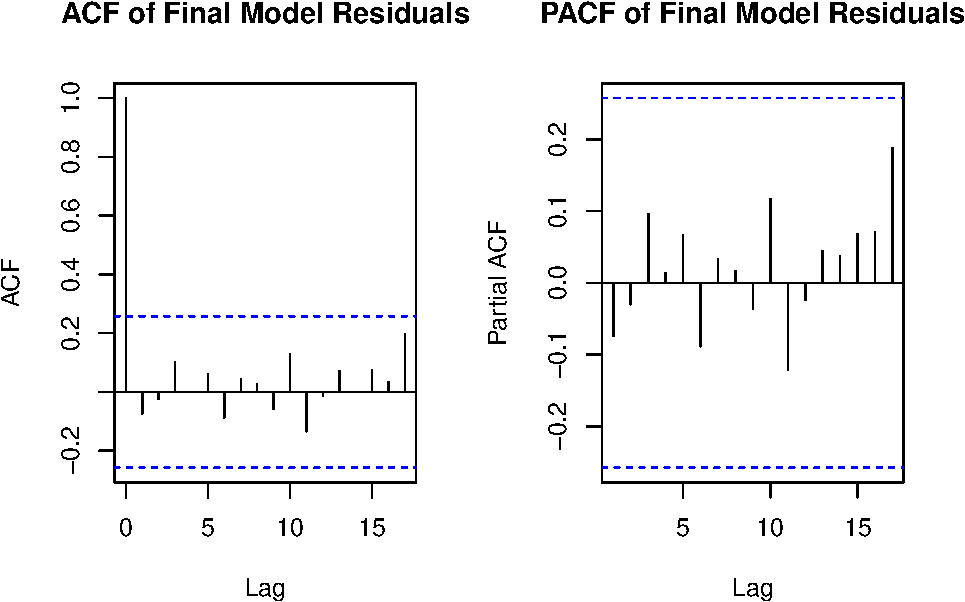
\includegraphics[keepaspectratio]{final_imports_files/figure-latex/unnamed-chunk-7-2.pdf}}

\begin{Shaded}
\begin{Highlighting}[]
\FunctionTok{par}\NormalTok{(}\AttributeTok{mfrow =} \FunctionTok{c}\NormalTok{(}\DecValTok{1}\NormalTok{, }\DecValTok{1}\NormalTok{))  }\CommentTok{\# Reset layout}

\FunctionTok{cat}\NormalTok{(}\StringTok{"}\SpecialCharTok{\textbackslash{}n}\StringTok{Diagnostic Tests:}\SpecialCharTok{\textbackslash{}n}\StringTok{"}\NormalTok{)}
\end{Highlighting}
\end{Shaded}

\begin{verbatim}
## 
## Diagnostic Tests:
\end{verbatim}

\begin{Shaded}
\begin{Highlighting}[]
\CommentTok{\# 1. Ljung{-}Box test}
\NormalTok{ljung }\OtherTok{\textless{}{-}} \FunctionTok{Box.test}\NormalTok{(residuals\_final, }\AttributeTok{lag =} \DecValTok{10}\NormalTok{, }\AttributeTok{type =} \StringTok{"Ljung{-}Box"}\NormalTok{)}
\FunctionTok{cat}\NormalTok{(}\StringTok{"Ljung{-}Box test p{-}value:"}\NormalTok{, }\FunctionTok{round}\NormalTok{(ljung}\SpecialCharTok{$}\NormalTok{p.value, }\DecValTok{4}\NormalTok{), }
    \FunctionTok{ifelse}\NormalTok{(ljung}\SpecialCharTok{$}\NormalTok{p.value }\SpecialCharTok{\textgreater{}} \FloatTok{0.05}\NormalTok{, }\StringTok{"(PASS)"}\NormalTok{, }\StringTok{"(FAIL)"}\NormalTok{), }\StringTok{"}\SpecialCharTok{\textbackslash{}n}\StringTok{"}\NormalTok{)}
\end{Highlighting}
\end{Shaded}

\begin{verbatim}
## Ljung-Box test p-value: 0.9723 (PASS)
\end{verbatim}

\begin{Shaded}
\begin{Highlighting}[]
\CommentTok{\# 2. Normality test}
\CommentTok{\# this does not violate model assumptions, but it violates confidence interval assumptions}
\NormalTok{shapiro }\OtherTok{\textless{}{-}} \FunctionTok{shapiro.test}\NormalTok{(residuals\_final)}
\FunctionTok{cat}\NormalTok{(}\StringTok{"Shapiro{-}Wilk test p{-}value:"}\NormalTok{, }\FunctionTok{round}\NormalTok{(shapiro}\SpecialCharTok{$}\NormalTok{p.value, }\DecValTok{4}\NormalTok{), }
    \FunctionTok{ifelse}\NormalTok{(shapiro}\SpecialCharTok{$}\NormalTok{p.value }\SpecialCharTok{\textgreater{}} \FloatTok{0.05}\NormalTok{, }\StringTok{"(PASS)"}\NormalTok{, }\StringTok{"(FAIL)"}\NormalTok{), }\StringTok{"}\SpecialCharTok{\textbackslash{}n}\StringTok{"}\NormalTok{)}
\end{Highlighting}
\end{Shaded}

\begin{verbatim}
## Shapiro-Wilk test p-value: 0.0258 (FAIL)
\end{verbatim}

\begin{Shaded}
\begin{Highlighting}[]
\CommentTok{\# 3. ARCH test}
\NormalTok{arch }\OtherTok{\textless{}{-}} \FunctionTok{Box.test}\NormalTok{(residuals\_final}\SpecialCharTok{\^{}}\DecValTok{2}\NormalTok{, }\AttributeTok{lag =} \DecValTok{5}\NormalTok{, }\AttributeTok{type =} \StringTok{"Ljung{-}Box"}\NormalTok{)}
\FunctionTok{cat}\NormalTok{(}\StringTok{"ARCH test p{-}value:"}\NormalTok{, }\FunctionTok{round}\NormalTok{(arch}\SpecialCharTok{$}\NormalTok{p.value, }\DecValTok{4}\NormalTok{), }
    \FunctionTok{ifelse}\NormalTok{(arch}\SpecialCharTok{$}\NormalTok{p.value }\SpecialCharTok{\textgreater{}} \FloatTok{0.05}\NormalTok{, }\StringTok{"(PASS)"}\NormalTok{, }\StringTok{"(FAIL)"}\NormalTok{), }\StringTok{"}\SpecialCharTok{\textbackslash{}n}\StringTok{"}\NormalTok{)}
\end{Highlighting}
\end{Shaded}

\begin{verbatim}
## ARCH test p-value: 0.9727 (PASS)
\end{verbatim}

\begin{Shaded}
\begin{Highlighting}[]
\FunctionTok{cat}\NormalTok{(}\StringTok{"}\SpecialCharTok{\textbackslash{}n}\StringTok{Slight non{-}normality detected but acceptable for ARIMA modeling}\SpecialCharTok{\textbackslash{}n}\StringTok{"}\NormalTok{)}
\end{Highlighting}
\end{Shaded}

\begin{verbatim}
## 
## Slight non-normality detected but acceptable for ARIMA modeling
\end{verbatim}

\begin{Shaded}
\begin{Highlighting}[]
\FunctionTok{cat}\NormalTok{(}\StringTok{"Q{-}Q plot shows approximate normality with minor tail deviations}\SpecialCharTok{\textbackslash{}n\textbackslash{}n}\StringTok{"}\NormalTok{)}
\end{Highlighting}
\end{Shaded}

\begin{verbatim}
## Q-Q plot shows approximate normality with minor tail deviations
\end{verbatim}

\begin{Shaded}
\begin{Highlighting}[]
\CommentTok{\# STEP 5: Forecast with Inverse Transformation}
\NormalTok{forecast\_result }\OtherTok{\textless{}{-}} \FunctionTok{forecast}\NormalTok{(final\_model, }\AttributeTok{h =} \DecValTok{3}\NormalTok{)}
\NormalTok{lambda }\OtherTok{\textless{}{-}} \FloatTok{0.1}
\CommentTok{\# Inverse Box{-}Cox transformation}
\NormalTok{forecast\_original }\OtherTok{\textless{}{-}}\NormalTok{ (lambda }\SpecialCharTok{*}\NormalTok{ forecast\_result}\SpecialCharTok{$}\NormalTok{mean }\SpecialCharTok{+} \DecValTok{1}\NormalTok{)}\SpecialCharTok{\^{}}\NormalTok{(}\DecValTok{1}\SpecialCharTok{/}\NormalTok{lambda)}
\NormalTok{lower\_original }\OtherTok{\textless{}{-}}\NormalTok{ (lambda }\SpecialCharTok{*}\NormalTok{ forecast\_result}\SpecialCharTok{$}\NormalTok{lower }\SpecialCharTok{+} \DecValTok{1}\NormalTok{)}\SpecialCharTok{\^{}}\NormalTok{(}\DecValTok{1}\SpecialCharTok{/}\NormalTok{lambda)}
\NormalTok{upper\_original }\OtherTok{\textless{}{-}}\NormalTok{ (lambda }\SpecialCharTok{*}\NormalTok{ forecast\_result}\SpecialCharTok{$}\NormalTok{upper }\SpecialCharTok{+} \DecValTok{1}\NormalTok{)}\SpecialCharTok{\^{}}\NormalTok{(}\DecValTok{1}\SpecialCharTok{/}\NormalTok{lambda)}
\FunctionTok{cat}\NormalTok{(}\StringTok{"1{-}step ahead forecast (original Imports scale):"}\NormalTok{, }\FunctionTok{round}\NormalTok{(forecast\_original[}\DecValTok{1}\NormalTok{], }\DecValTok{2}\NormalTok{), }\StringTok{"Imports}\SpecialCharTok{\textbackslash{}n}\StringTok{"}\NormalTok{)}
\end{Highlighting}
\end{Shaded}

\begin{verbatim}
## 1-step ahead forecast (original Imports scale): 403.83 Imports
\end{verbatim}

\begin{Shaded}
\begin{Highlighting}[]
\FunctionTok{cat}\NormalTok{(}\StringTok{"95\% prediction interval: ["}\NormalTok{, }\FunctionTok{round}\NormalTok{(lower\_original[}\DecValTok{1}\NormalTok{,}\DecValTok{2}\NormalTok{], }\DecValTok{2}\NormalTok{), }\StringTok{","}\NormalTok{, }
    \FunctionTok{round}\NormalTok{(upper\_original[}\DecValTok{1}\NormalTok{,}\DecValTok{2}\NormalTok{], }\DecValTok{2}\NormalTok{), }\StringTok{"] Imports}\SpecialCharTok{\textbackslash{}n\textbackslash{}n}\StringTok{"}\NormalTok{)}
\end{Highlighting}
\end{Shaded}

\begin{verbatim}
## 95% prediction interval: [ 226.32 , 698.07 ] Imports
\end{verbatim}

\begin{Shaded}
\begin{Highlighting}[]
\FunctionTok{cat}\NormalTok{(}\StringTok{"FINAL MODEL: ARIMA(0,1,0) for Box{-}Cox transformed Imports}\SpecialCharTok{\textbackslash{}n}\StringTok{"}\NormalTok{)}
\end{Highlighting}
\end{Shaded}

\begin{verbatim}
## FINAL MODEL: ARIMA(0,1,0) for Box-Cox transformed Imports
\end{verbatim}

\section{Forecast next 10 periods using the best
model}\label{forecast-next-10-periods-using-the-best-model}

\begin{Shaded}
\begin{Highlighting}[]
\NormalTok{forecast\_horizon }\OtherTok{\textless{}{-}} \DecValTok{10}
\NormalTok{imports\_forecast }\OtherTok{\textless{}{-}} \FunctionTok{forecast}\NormalTok{(final\_model, }\AttributeTok{h =}\NormalTok{ forecast\_horizon)}

\CommentTok{\# Plot the forecast}
\FunctionTok{autoplot}\NormalTok{(imports\_forecast) }\SpecialCharTok{+}
  \FunctionTok{ggtitle}\NormalTok{(}\StringTok{"ARIMA Forecast of Imports (in Millions }\SpecialCharTok{\textbackslash{}\textbackslash{}}\StringTok{$)"}\NormalTok{) }\SpecialCharTok{+}
  \FunctionTok{xlab}\NormalTok{(}\StringTok{"Year"}\NormalTok{) }\SpecialCharTok{+}
  \FunctionTok{ylab}\NormalTok{(}\StringTok{"Imports"}\NormalTok{) }\SpecialCharTok{+}
  \FunctionTok{theme\_minimal}\NormalTok{()}
\end{Highlighting}
\end{Shaded}

\pandocbounded{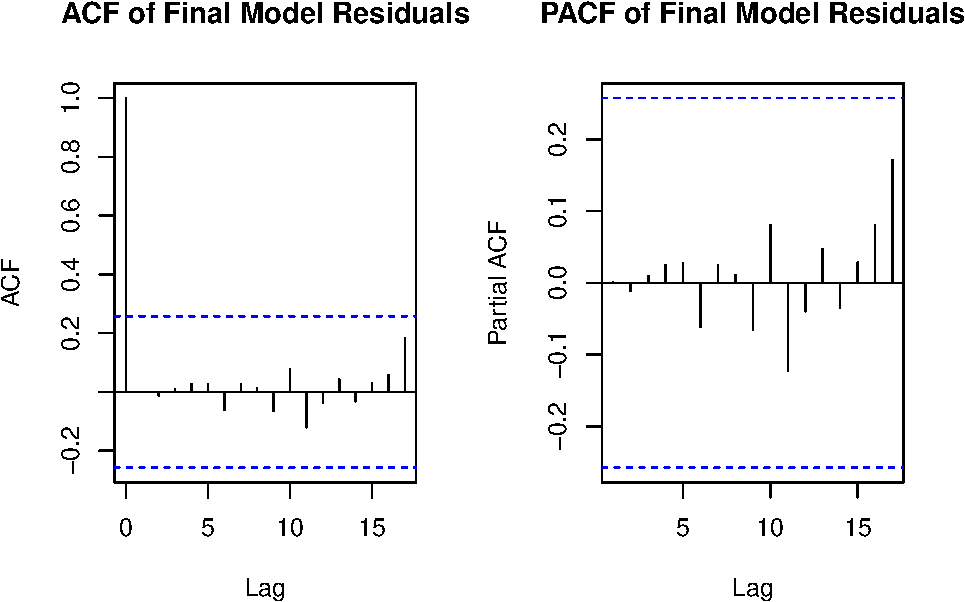
\includegraphics[keepaspectratio]{final_imports_files/figure-latex/unnamed-chunk-8-1.pdf}}

\end{document}
